% 12-minute talk. Compile on Overleaf (beamer). Numbers from ../report/numbers.tex.
\documentclass[aspectratio=169,10pt]{beamer}
\usetheme{default}
\setbeamertemplate{navigation symbols}{}
\setbeamertemplate{footline}[frame number]
\usepackage{graphicx,booktabs}
\graphicspath{{../report/figures/}}
% generated by report/make_numbers.py from results/tables -- do not edit
\newcommand{\NRecordings}{18}
\newcommand{\NTrialsSession}{288}
\newcommand{\NTrialsTotal}{5184}
\newcommand{\ExpertMin}{5}
\newcommand{\ExpertMax}{73}
\newcommand{\ExpertTotal}{488}
\newcommand{\ExpertPct}{9.4}
\newcommand{\CalibAFourT}{80}
\newcommand{\FilterTaps}{825}
\newcommand{\FilterLenS}{3.3}
\newcommand{\GainFiftyDefault}{-4.5}
\newcommand{\GainFifty}{-51}
\newcommand{\LineMax}{20}
\newcommand{\LineMaxRec}{S5 1test}
\newcommand{\IcaExclTwo}{17}
\newcommand{\IcaExclMax}{3}
\newcommand{\IcaMinScore}{0.55}
\newcommand{\FzEogRNone}{0.73}
\newcommand{\FzEogRReg}{0.08}
\newcommand{\FzEogRIca}{0.15}
\newcommand{\PtpMax}{142}
\newcommand{\PtpPctNineNineFive}{107}
\newcommand{\RegInjected}{6}
\newcommand{\RegInjectedExpert}{6}
\newcommand{\RegInjectedMax}{395}
\newcommand{\HeogPos}{17}
\newcommand{\HeogSig}{15}
\newcommand{\HeogDMax}{3.24}
\newcommand{\HeogOnsetMin}{192}
\newcommand{\HeogOnsetMax}{196}
\newcommand{\HeogPeak}{366}
\newcommand{\LatNegAny}{18}
\newcommand{\LatNegBeta}{18}
\newcommand{\WeakErd}{S2 0train, S5 0train, S5 1test, S7 0train}
\newcommand{\SNineHighP}{1.6e-19}
\newcommand{\AucEogNoneT}{0.86}
\newcommand{\AboveEogNoneT}{8}
\newcommand{\AucAllNoneT}{0.85}
\newcommand{\AboveAllNoneT}{8}
\newcommand{\AucAllRegT}{0.83}
\newcommand{\AboveAllRegT}{8}
\newcommand{\AucAllIcaT}{0.80}
\newcommand{\AboveAllIcaT}{8}
\newcommand{\AucPhysioNoneT}{0.77}
\newcommand{\AbovePhysioNoneT}{8}
\newcommand{\AucPhysioRegT}{0.77}
\newcommand{\AbovePhysioRegT}{8}
\newcommand{\AucPhysioIcaT}{0.77}
\newcommand{\AbovePhysioIcaT}{8}
\newcommand{\AucProneNoneT}{0.57}
\newcommand{\AboveProneNoneT}{3}
\newcommand{\AucProneRegT}{0.58}
\newcommand{\AboveProneRegT}{3}
\newcommand{\AucProneIcaT}{0.56}
\newcommand{\AboveProneIcaT}{3}
\newcommand{\AucEogNoneE}{0.87}
\newcommand{\AboveEogNoneE}{9}
\newcommand{\AucAllNoneE}{0.86}
\newcommand{\AboveAllNoneE}{8}
\newcommand{\AucAllRegE}{0.83}
\newcommand{\AboveAllRegE}{7}
\newcommand{\AucAllIcaE}{0.89}
\newcommand{\AboveAllIcaE}{8}
\newcommand{\AucPhysioNoneE}{0.80}
\newcommand{\AbovePhysioNoneE}{8}
\newcommand{\AucPhysioRegE}{0.80}
\newcommand{\AbovePhysioRegE}{9}
\newcommand{\AucPhysioIcaE}{0.87}
\newcommand{\AbovePhysioIcaE}{7}
\newcommand{\AucProneNoneE}{0.59}
\newcommand{\AboveProneNoneE}{3}
\newcommand{\AucProneRegE}{0.53}
\newcommand{\AboveProneRegE}{2}
\newcommand{\AucProneIcaE}{0.54}
\newcommand{\AboveProneIcaE}{4}
\newcommand{\BaccEogNone}{0.56}
\newcommand{\BaccAllNone}{0.59}
\newcommand{\BaccAllIca}{0.58}
\newcommand{\BaccPhysioNone}{0.59}
\newcommand{\BaccPhysioIca}{0.64}
\newcommand{\BaccProneNone}{0.34}
\newcommand{\BaccProneIca}{0.32}
\newcommand{\BaccChance}{0.29}
\newcommand{\NestedDiff}{0.007}
\newcommand{\XsEog}{0.84}
\newcommand{\XsAllNone}{0.86}
\newcommand{\XsAllIca}{0.89}
\newcommand{\HoneP}{0.002}
\newcommand{\HoneW}{45}
\newcommand{\HoneDelta}{0.36}
\newcommand{\HoneIqrLo}{0.27}
\newcommand{\HoneIqrHi}{0.47}
\newcommand{\HoneAbove}{8}
\newcommand{\HoneN}{9}
\newcommand{\HoneVerdict}{supported}
\newcommand{\HtwoPReg}{0.633}
\newcommand{\HtwoPholmReg}{1.000}
\newcommand{\HtwoDeltaReg}{-0.002}
\newcommand{\HtwoRhoReg}{0.35}
\newcommand{\HtwoRhoPReg}{0.356}
\newcommand{\HtwoPIca}{0.633}
\newcommand{\HtwoPholmIca}{1.000}
\newcommand{\HtwoDeltaIca}{-0.002}
\newcommand{\HtwoRhoIca}{-0.42}
\newcommand{\HtwoRhoPIca}{0.265}
\newcommand{\HtwoVerdict}{not supported}
\newcommand{\HthreeP}{0.752}
\newcommand{\HthreeDropPhysio}{-0.010}
\newcommand{\HthreeDropProne}{-0.057}
\newcommand{\HthreeShareNone}{24.8}
\newcommand{\HthreeShareIca}{27.6}
\newcommand{\HthreeShareP}{0.125}
\newcommand{\HthreeVerdict}{not supported}
\newcommand{\RobHoneAll}{all}
\newcommand{\RobHoneN}{5}
\newcommand{\RobHtwoAny}{0}
\newcommand{\RobHtwoN}{10}
\newcommand{\ExPReg}{0.125}
\newcommand{\ExPholmReg}{0.375}
\newcommand{\ExAucReg}{0.67}
\newcommand{\ExDeltaReg}{0.013}
\newcommand{\ExRhoReg}{0.98}
\newcommand{\ExRhoPReg}{1.9e-06}
\newcommand{\ExPIca}{0.590}
\newcommand{\ExPholmIca}{0.652}
\newcommand{\ExAucIca}{0.71}
\newcommand{\ExDeltaIca}{-0.025}
\newcommand{\ExRhoIca}{0.85}
\newcommand{\ExRhoPIca}{0.004}
\newcommand{\ExAucNone}{0.70}
\newcommand{\ExAboveNone}{8}
\newcommand{\TimeDecode}{6.2}
\newcommand{\NPermH}{100}

\title{Do eye movements drive motor-imagery decoding on BCI~IV~2a?}
\author{Chidiadi Bethel Mba \and Sungkar Bolat \and Beibars Ybraiakhyn \and Ramazan Zypayev}
\institute{ROBT613 Brain Machine Interface, Nazarbayev University}
\date{}
\begin{document}
\frame{\titlepage}

\begin{frame}{Question and pre-registered hypotheses}
\begin{itemize}
\item The 2a cue is an arrow pointing toward the task (left, right, down, up)
\item H1 \quad EOG alone decodes left vs right above chance in most subjects
\item H2 \quad Removing ocular activity lowers EEG decoding, more where H1 is strong
\item H3 \quad Cleaning moves weight from frontal / artifact bands to central mu and beta
\item Decision rules fixed before running FULL (Wilcoxon, own permutation null, $n=9$)
\end{itemize}
\end{frame}

\begin{frame}{Stage 1 \quad Data audit}
\begin{columns}
\column{0.5\textwidth}
\begin{itemize}\small
\item \NRecordings{} recordings, \NTrialsSession{} trials each, 22 EEG + 3 EOG, 250 Hz
\item Annotation = cue onset (checked for every trial)
\item Recovered from the source files: expert artifact flags (\ExpertMin{}--\ExpertMax{} per session) and EOG calibration runs
\end{itemize}
\column{0.5\textwidth}
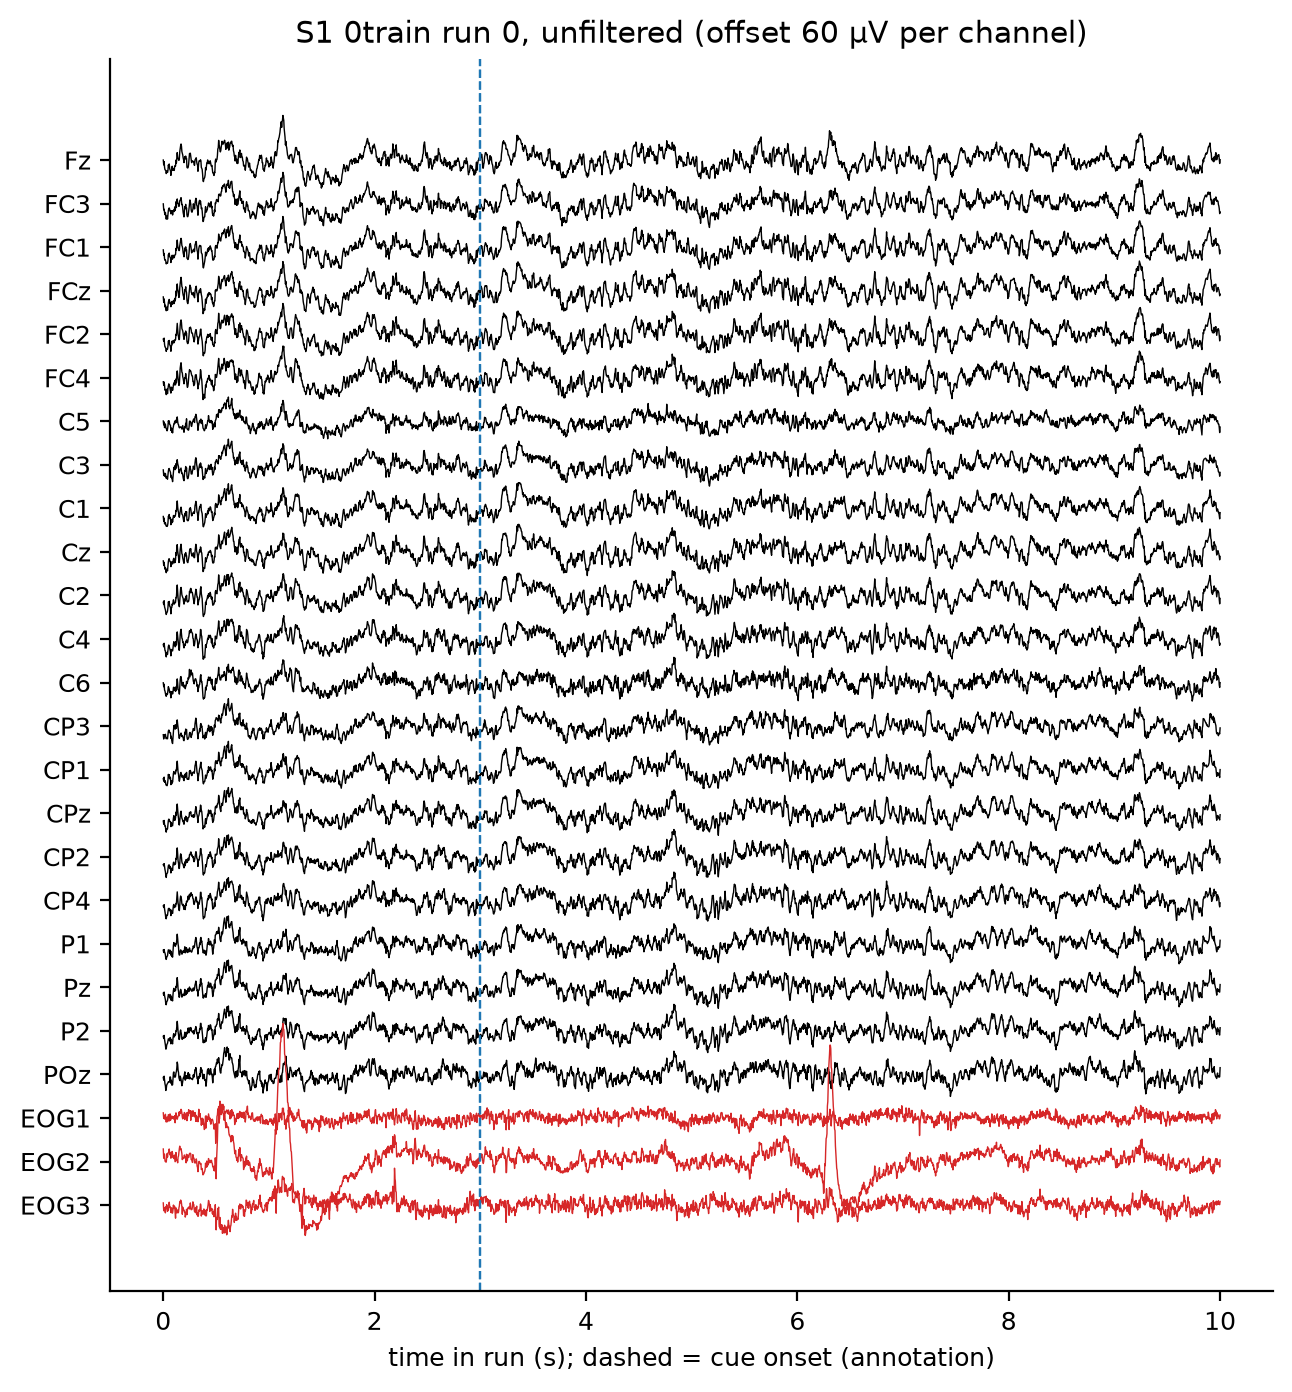
\includegraphics[width=\linewidth]{fig_1a_raw_segment.png}
\end{columns}
\end{frame}

\begin{frame}{Stage 2 \quad Signal inspection and filtering}
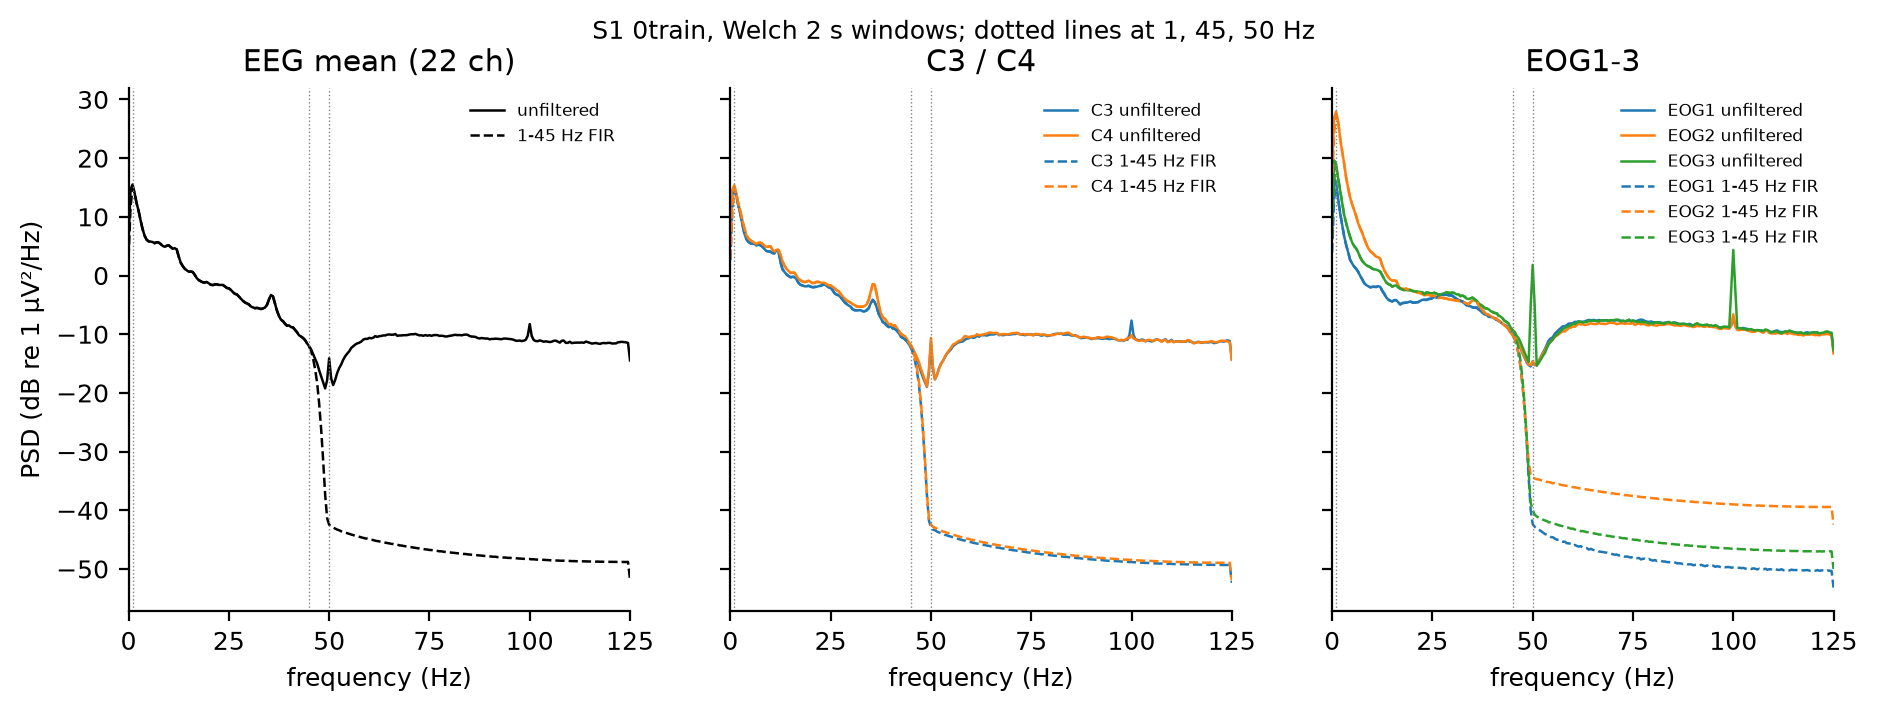
\includegraphics[width=\linewidth]{fig_2a_psd_before_after.png}
\small 1--45 Hz FIR. Default design gives only \GainFiftyDefault{} dB at 50 Hz, ours \GainFifty{} dB, so no notch needed.
\end{frame}

\begin{frame}{Stage 3 \quad Artifact handling}
\begin{columns}
\column{0.55\textwidth}
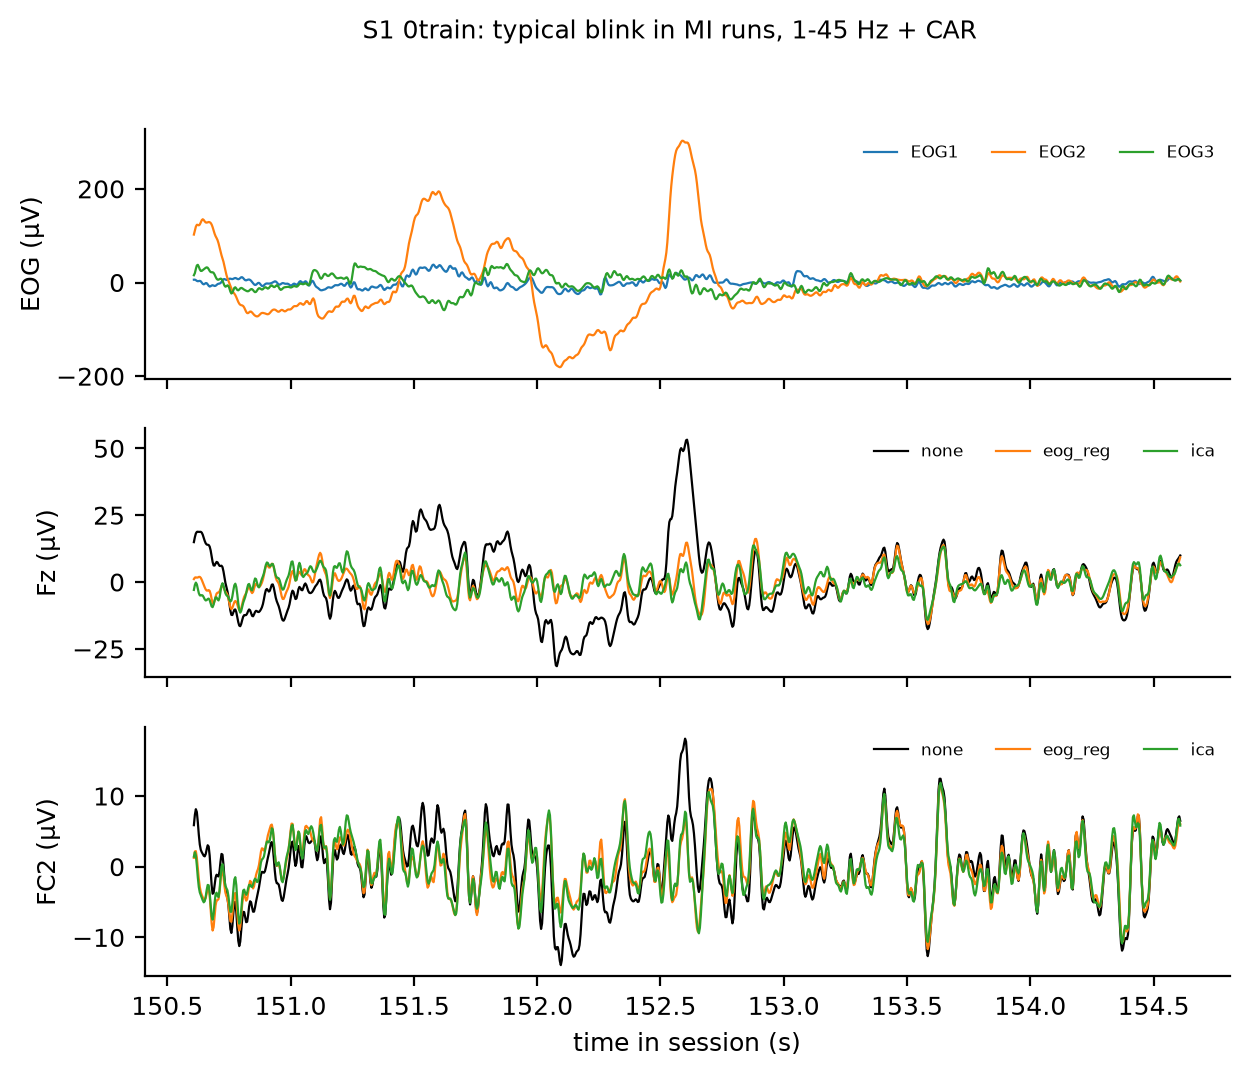
\includegraphics[width=\linewidth]{fig_3b_eog_regression_before_after.png}
\column{0.45\textwidth}
\begin{itemize}\small
\item none = filter + CAR, eog\_reg, ica (20 comps, $|r|\ge0.5$)
\item Both fitted on calibration runs, never on MI trials
\item Fz--EOG2 $|r|$ \FzEogRNone{} $\to$ \FzEogRReg{} / \FzEogRIca{}
\item No rejection (max \PtpMax{} $\mu$V), same epochs in all conditions
\end{itemize}
\end{columns}
\end{frame}

\begin{frame}{Stage 4 \quad The confound exists before any classifier}
\centering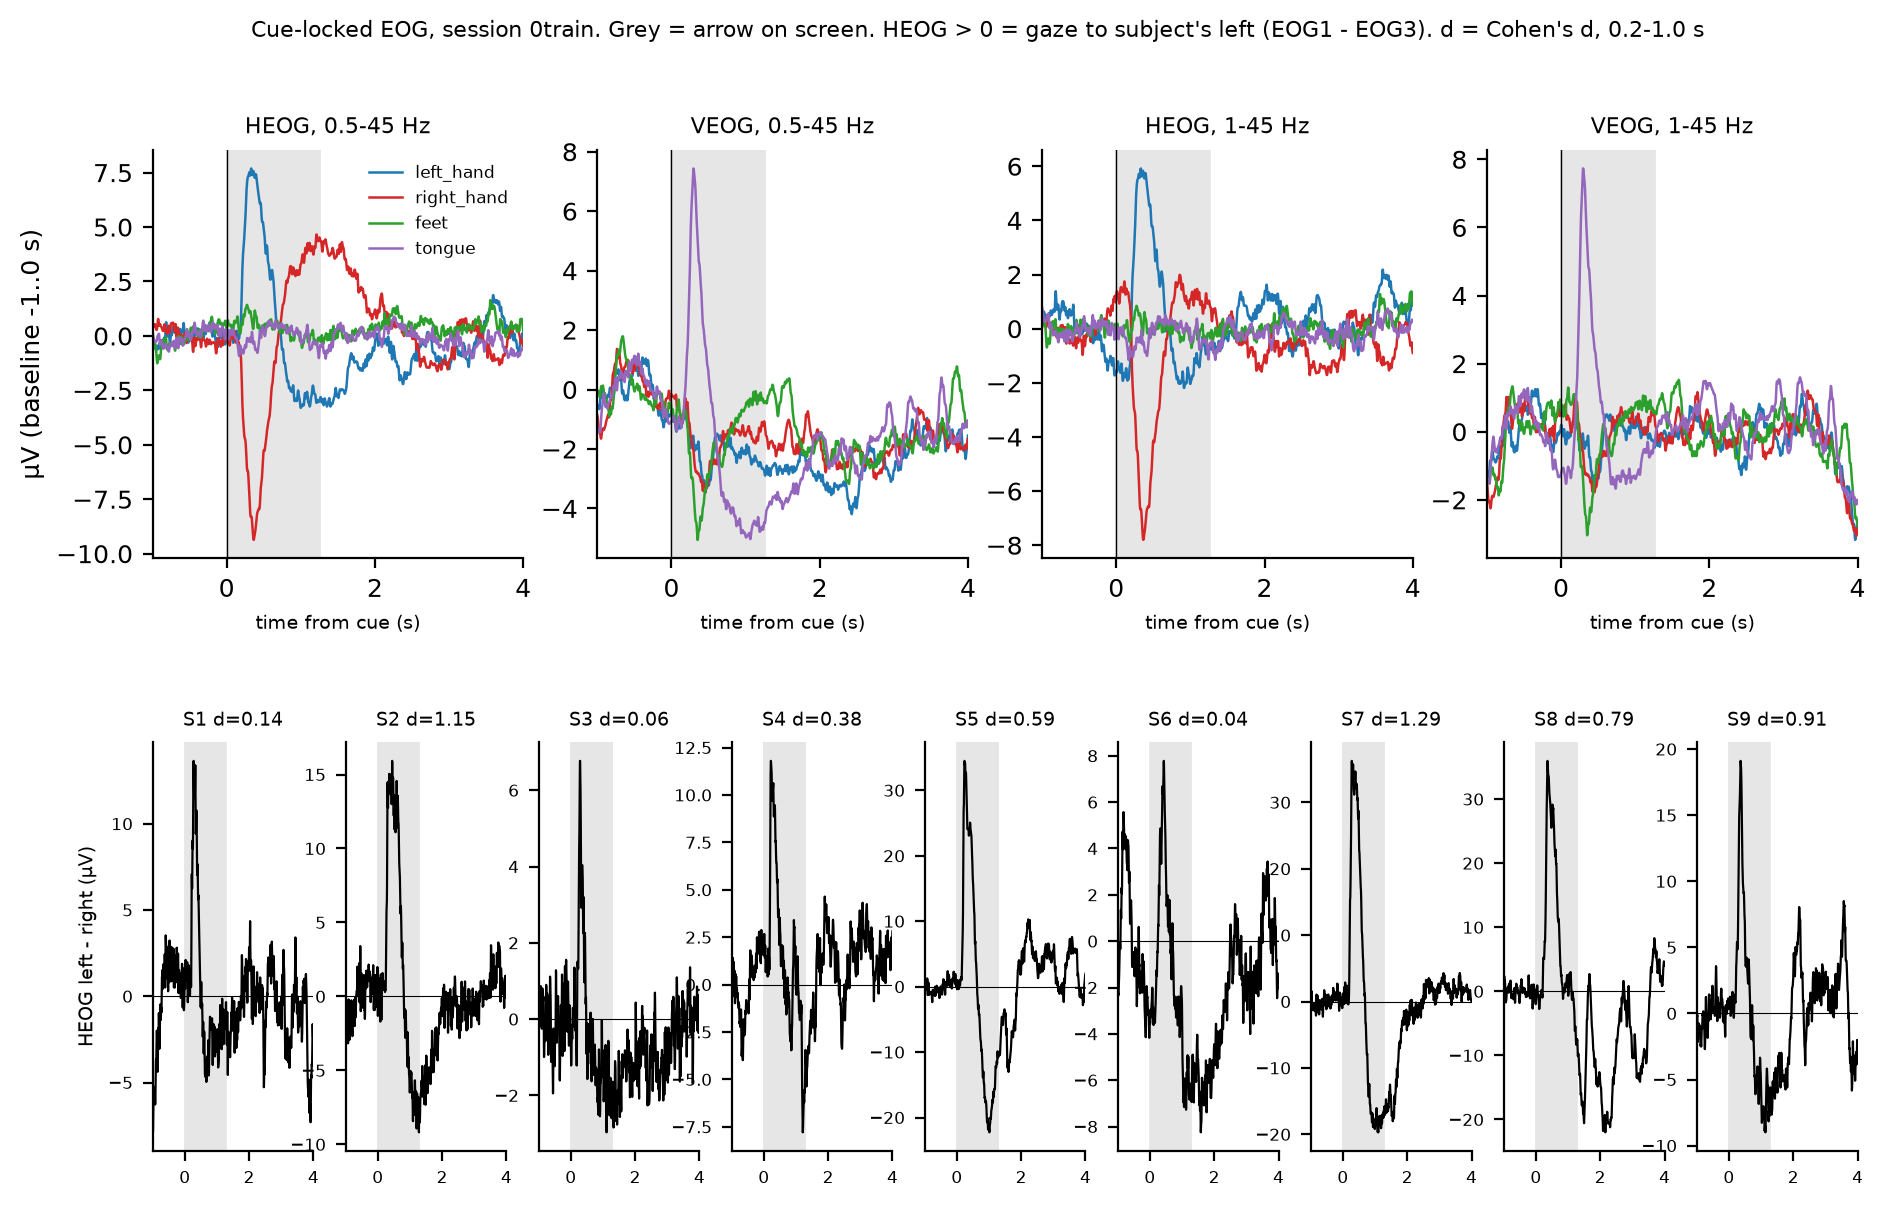
\includegraphics[height=0.74\textheight,width=\linewidth,keepaspectratio]{fig_4c_eog_evoked_by_class.png}

\raggedright
\small Gaze follows the arrow in \HeogPos{}/\NRecordings{} recordings, onset \HeogOnsetMin{}--\HeogOnsetMax{} ms after the cue
\end{frame}

\begin{frame}{Stage 5--6 \quad Features, classifiers, honest evaluation}
\begin{columns}
\column{0.4\textwidth}
\begin{itemize}\small
\item Log band power (MI window) and amplitude bins
\item 4 feature sets $\times$ 3 cleanings $\times$ logreg / sLDA
\item Leave-one-run-out CV, within-run permutation null for every row
\item Leakage test in the test suite
\end{itemize}
\column{0.6\textwidth}
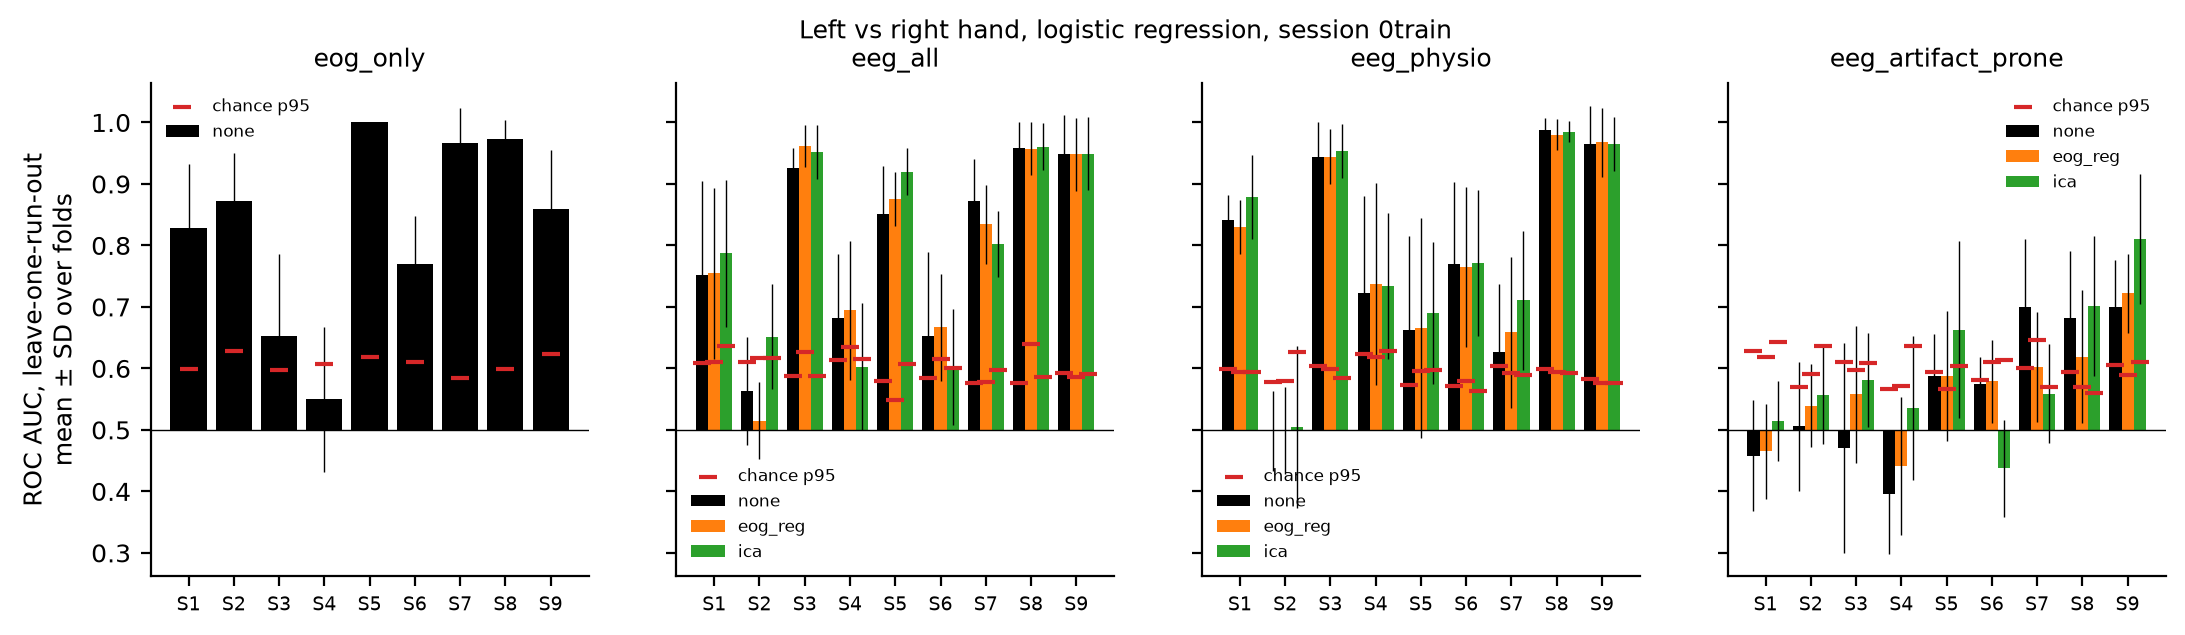
\includegraphics[width=\linewidth]{fig_6a_auc_per_subject_by_condition.png}
\end{columns}
\end{frame}

\begin{frame}{Stage 7 \quad H1 \HoneVerdict{}}
\begin{columns}
\column{0.55\textwidth}
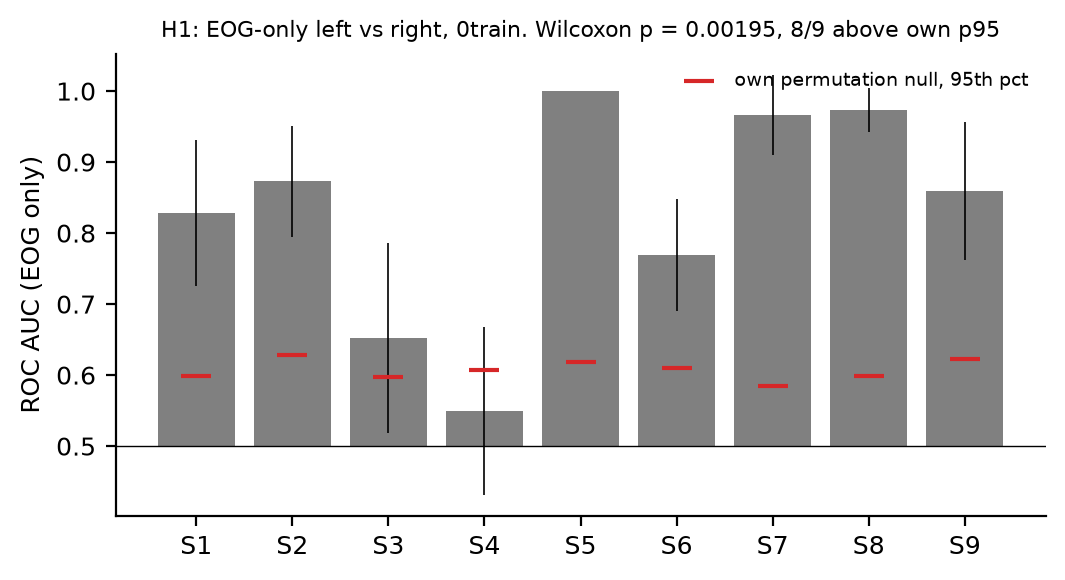
\includegraphics[width=\linewidth]{fig_7a_eog_only_auc_vs_null.png}
\column{0.45\textwidth}
\begin{itemize}\small
\item EOG-only median AUC \AucEogNoneT{} (0train), \AucEogNoneE{} (1test)
\item \HoneAbove{}/\HoneN{} above own null, Wilcoxon $p=\HoneP{}$
\item Holds in \RobHoneAll{} \RobHoneN{} robustness analyses
\end{itemize}
\end{columns}
\end{frame}

\begin{frame}{Stage 7 \quad H2 and H3 \HtwoVerdict{}}
\begin{columns}
\column{0.5\textwidth}
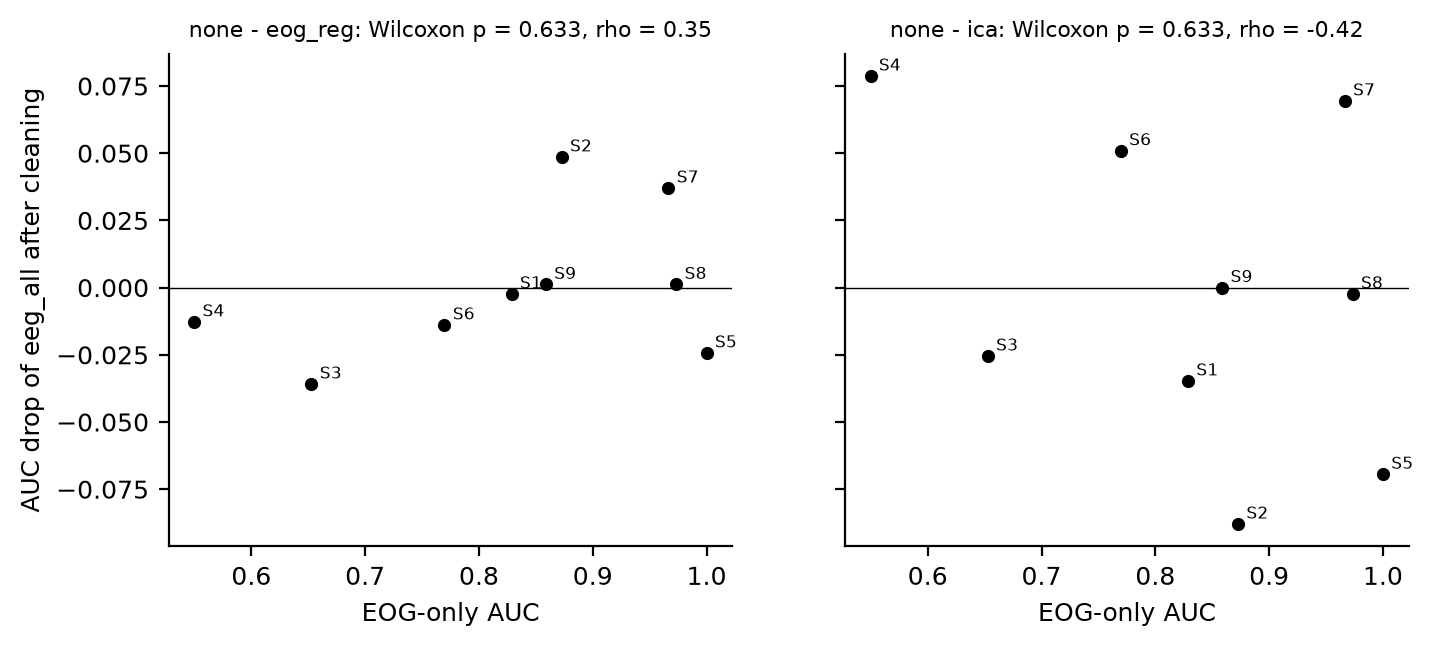
\includegraphics[width=\linewidth]{fig_7b_auc_drop_vs_eog_auc.png}
\column{0.5\textwidth}
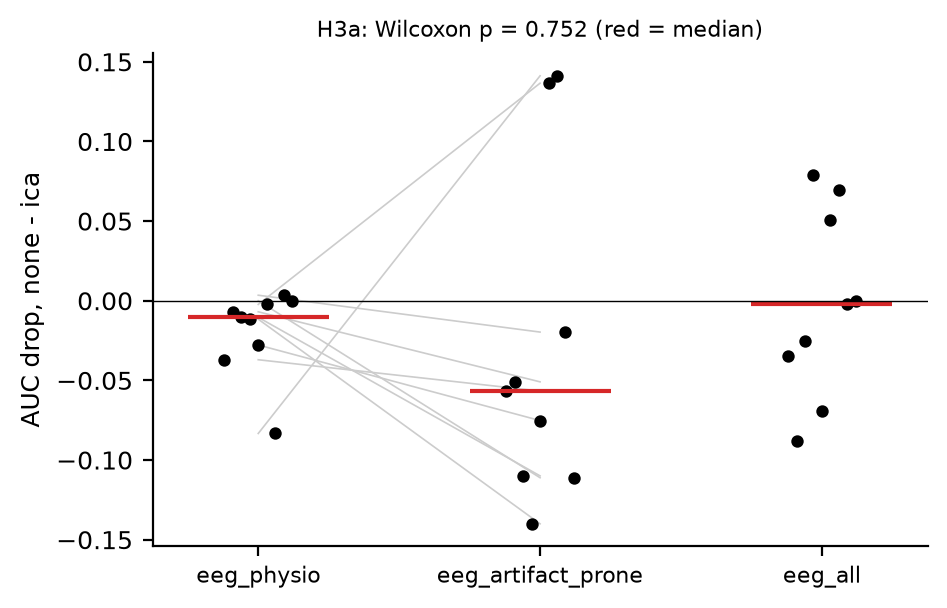
\includegraphics[width=\linewidth]{fig_7d_delta_auc_by_feature_set.png}
\end{columns}
\small eeg\_all AUC \AucAllNoneT{} $\to$ \AucAllRegT{} / \AucAllIcaT{}, $p=\HtwoPReg{}$ / \HtwoPIca{}. Artifact-prone set does not lose more ($p=\HthreeP{}$).
\end{frame}

\begin{frame}{Exploratory \quad where the risk lies}
\begin{columns}
\column{0.5\textwidth}
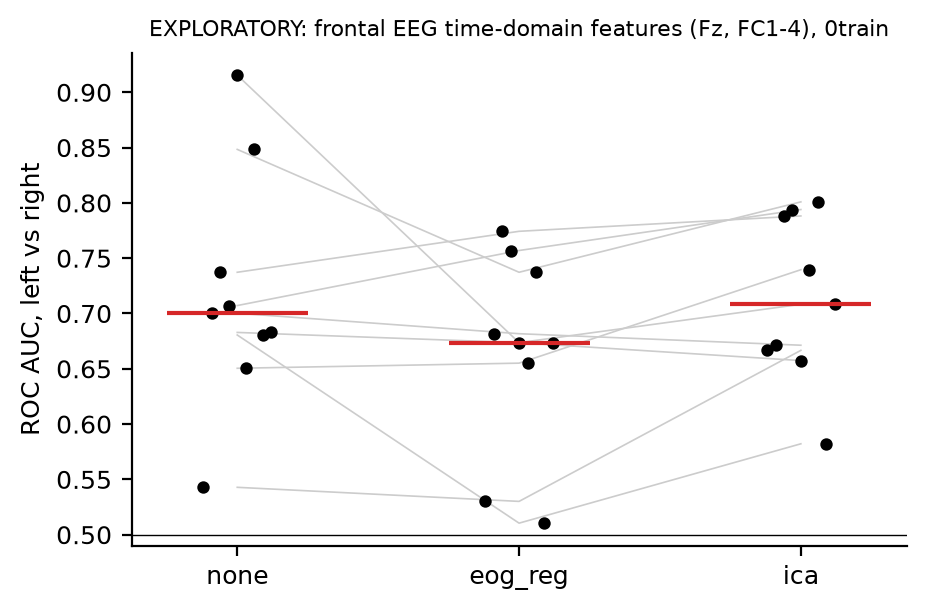
\includegraphics[width=\linewidth]{fig_7e_exploratory_frontal_amplitude.png}
\column{0.5\textwidth}
\begin{itemize}\small
\item Not pre-registered
\item Frontal EEG time-domain features, AUC \ExAucNone{} $\to$ \ExAucReg{} / \ExAucIca{}
\item The confound is a time-domain event, band power in the MI window does not pick it up
\end{itemize}
\end{columns}
\end{frame}

\begin{frame}{Limits and take-home}
\begin{itemize}
\item Offline, $n=9$, low power for small cleaning effects
\item Regression and ICA target eyes, not EMG (tongue)
\item Cleaning is partial at frontal sites
\item Gaze shift is a reflex to the cue, not cheating
\item Take-home \quad report an EOG-only baseline next to any 2a score that uses EOG, frontal time-domain features or cue-overlapping windows
\end{itemize}
\end{frame}
\end{document}
